% Options for packages loaded elsewhere
\PassOptionsToPackage{unicode}{hyperref}
\PassOptionsToPackage{hyphens}{url}
%
\documentclass[
]{article}
\usepackage{lmodern}
\usepackage{amssymb,amsmath}
\usepackage{ifxetex,ifluatex}
\ifnum 0\ifxetex 1\fi\ifluatex 1\fi=0 % if pdftex
  \usepackage[T1]{fontenc}
  \usepackage[utf8]{inputenc}
  \usepackage{textcomp} % provide euro and other symbols
\else % if luatex or xetex
  \usepackage{unicode-math}
  \defaultfontfeatures{Scale=MatchLowercase}
  \defaultfontfeatures[\rmfamily]{Ligatures=TeX,Scale=1}
\fi
% Use upquote if available, for straight quotes in verbatim environments
\IfFileExists{upquote.sty}{\usepackage{upquote}}{}
\IfFileExists{microtype.sty}{% use microtype if available
  \usepackage[]{microtype}
  \UseMicrotypeSet[protrusion]{basicmath} % disable protrusion for tt fonts
}{}
\makeatletter
\@ifundefined{KOMAClassName}{% if non-KOMA class
  \IfFileExists{parskip.sty}{%
    \usepackage{parskip}
  }{% else
    \setlength{\parindent}{0pt}
    \setlength{\parskip}{6pt plus 2pt minus 1pt}}
}{% if KOMA class
  \KOMAoptions{parskip=half}}
\makeatother
\usepackage{xcolor}
\IfFileExists{xurl.sty}{\usepackage{xurl}}{} % add URL line breaks if available
\IfFileExists{bookmark.sty}{\usepackage{bookmark}}{\usepackage{hyperref}}
\hypersetup{
  pdftitle={Monty Hall Simulation},
  pdfauthor={coop711},
  hidelinks,
  pdfcreator={LaTeX via pandoc}}
\urlstyle{same} % disable monospaced font for URLs
\usepackage[margin=1in]{geometry}
\usepackage{color}
\usepackage{fancyvrb}
\newcommand{\VerbBar}{|}
\newcommand{\VERB}{\Verb[commandchars=\\\{\}]}
\DefineVerbatimEnvironment{Highlighting}{Verbatim}{commandchars=\\\{\}}
% Add ',fontsize=\small' for more characters per line
\usepackage{framed}
\definecolor{shadecolor}{RGB}{248,248,248}
\newenvironment{Shaded}{\begin{snugshade}}{\end{snugshade}}
\newcommand{\AlertTok}[1]{\textcolor[rgb]{0.94,0.16,0.16}{#1}}
\newcommand{\AnnotationTok}[1]{\textcolor[rgb]{0.56,0.35,0.01}{\textbf{\textit{#1}}}}
\newcommand{\AttributeTok}[1]{\textcolor[rgb]{0.77,0.63,0.00}{#1}}
\newcommand{\BaseNTok}[1]{\textcolor[rgb]{0.00,0.00,0.81}{#1}}
\newcommand{\BuiltInTok}[1]{#1}
\newcommand{\CharTok}[1]{\textcolor[rgb]{0.31,0.60,0.02}{#1}}
\newcommand{\CommentTok}[1]{\textcolor[rgb]{0.56,0.35,0.01}{\textit{#1}}}
\newcommand{\CommentVarTok}[1]{\textcolor[rgb]{0.56,0.35,0.01}{\textbf{\textit{#1}}}}
\newcommand{\ConstantTok}[1]{\textcolor[rgb]{0.00,0.00,0.00}{#1}}
\newcommand{\ControlFlowTok}[1]{\textcolor[rgb]{0.13,0.29,0.53}{\textbf{#1}}}
\newcommand{\DataTypeTok}[1]{\textcolor[rgb]{0.13,0.29,0.53}{#1}}
\newcommand{\DecValTok}[1]{\textcolor[rgb]{0.00,0.00,0.81}{#1}}
\newcommand{\DocumentationTok}[1]{\textcolor[rgb]{0.56,0.35,0.01}{\textbf{\textit{#1}}}}
\newcommand{\ErrorTok}[1]{\textcolor[rgb]{0.64,0.00,0.00}{\textbf{#1}}}
\newcommand{\ExtensionTok}[1]{#1}
\newcommand{\FloatTok}[1]{\textcolor[rgb]{0.00,0.00,0.81}{#1}}
\newcommand{\FunctionTok}[1]{\textcolor[rgb]{0.00,0.00,0.00}{#1}}
\newcommand{\ImportTok}[1]{#1}
\newcommand{\InformationTok}[1]{\textcolor[rgb]{0.56,0.35,0.01}{\textbf{\textit{#1}}}}
\newcommand{\KeywordTok}[1]{\textcolor[rgb]{0.13,0.29,0.53}{\textbf{#1}}}
\newcommand{\NormalTok}[1]{#1}
\newcommand{\OperatorTok}[1]{\textcolor[rgb]{0.81,0.36,0.00}{\textbf{#1}}}
\newcommand{\OtherTok}[1]{\textcolor[rgb]{0.56,0.35,0.01}{#1}}
\newcommand{\PreprocessorTok}[1]{\textcolor[rgb]{0.56,0.35,0.01}{\textit{#1}}}
\newcommand{\RegionMarkerTok}[1]{#1}
\newcommand{\SpecialCharTok}[1]{\textcolor[rgb]{0.00,0.00,0.00}{#1}}
\newcommand{\SpecialStringTok}[1]{\textcolor[rgb]{0.31,0.60,0.02}{#1}}
\newcommand{\StringTok}[1]{\textcolor[rgb]{0.31,0.60,0.02}{#1}}
\newcommand{\VariableTok}[1]{\textcolor[rgb]{0.00,0.00,0.00}{#1}}
\newcommand{\VerbatimStringTok}[1]{\textcolor[rgb]{0.31,0.60,0.02}{#1}}
\newcommand{\WarningTok}[1]{\textcolor[rgb]{0.56,0.35,0.01}{\textbf{\textit{#1}}}}
\usepackage{graphicx,grffile}
\makeatletter
\def\maxwidth{\ifdim\Gin@nat@width>\linewidth\linewidth\else\Gin@nat@width\fi}
\def\maxheight{\ifdim\Gin@nat@height>\textheight\textheight\else\Gin@nat@height\fi}
\makeatother
% Scale images if necessary, so that they will not overflow the page
% margins by default, and it is still possible to overwrite the defaults
% using explicit options in \includegraphics[width, height, ...]{}
\setkeys{Gin}{width=\maxwidth,height=\maxheight,keepaspectratio}
% Set default figure placement to htbp
\makeatletter
\def\fps@figure{htbp}
\makeatother
\setlength{\emergencystretch}{3em} % prevent overfull lines
\providecommand{\tightlist}{%
  \setlength{\itemsep}{0pt}\setlength{\parskip}{0pt}}
\setcounter{secnumdepth}{-\maxdimen} % remove section numbering

\title{Monty Hall Simulation}
\author{coop711}
\date{2020-11-23}

\begin{document}
\maketitle

\begin{flushleft}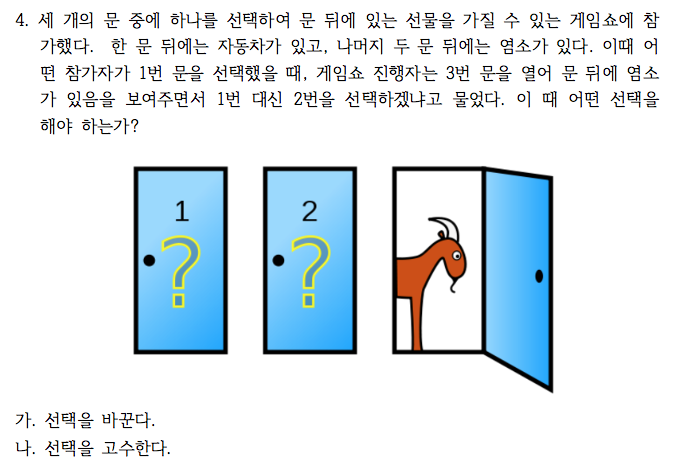
\includegraphics[width=0.65\linewidth]{../pics/Monty_Hall} \end{flushleft}

\hypertarget{single-trial}{%
\subsection{Single Trial}\label{single-trial}}

\begin{Shaded}
\begin{Highlighting}[]
\KeywordTok{set.seed}\NormalTok{(}\DecValTok{41}\NormalTok{)}
\NormalTok{monty_hall <-}\StringTok{ }\ControlFlowTok{function}\NormalTok{() \{}
\NormalTok{  key <-}\StringTok{ }\DecValTok{1}\OperatorTok{:}\DecValTok{3} \OperatorTok\StringTok{ }\KeywordTok{sample}\NormalTok{(}\DataTypeTok{size =} \DecValTok{1}\NormalTok{)}
\NormalTok{  goat <-}\StringTok{ }\DecValTok{1}\OperatorTok{:}\DecValTok{3} \OperatorTok\StringTok{ }\KeywordTok{setdiff}\NormalTok{(key)}
\NormalTok{  contestant <-}\StringTok{ }\DecValTok{1}\OperatorTok{:}\DecValTok{3} \OperatorTok\StringTok{ }\KeywordTok{sample}\NormalTok{(}\DataTypeTok{size =} \DecValTok{1}\NormalTok{)}
\NormalTok{  monty <-}\StringTok{ }\NormalTok{contestant }\OperatorTok
\StringTok{    `}\DataTypeTok{==}\StringTok{`}\NormalTok{ (key) }\OperatorTok
\StringTok{    }\KeywordTok{ifelse}\NormalTok{(goat }\OperatorTok\StringTok{ }\KeywordTok{sample}\NormalTok{(}\DataTypeTok{size =} \DecValTok{1}\NormalTok{), }
\NormalTok{           goat }\OperatorTok\StringTok{ }\KeywordTok{setdiff}\NormalTok{(contestant))}
  \ControlFlowTok{switch}\NormalTok{ <-}\StringTok{ }\DecValTok{1}\OperatorTok{:}\DecValTok{3} \OperatorTok\StringTok{ }\KeywordTok{setdiff}\NormalTok{(}\KeywordTok{c}\NormalTok{(contestant, monty))}
\NormalTok{  result <-}\StringTok{ }\ControlFlowTok{switch} \OperatorTok\StringTok{ }
\StringTok{    `}\DataTypeTok{==}\StringTok{`}\NormalTok{(key) }\OperatorTok
\StringTok{    }\KeywordTok{ifelse}\NormalTok{(}\StringTok{"Switching wins"}\NormalTok{, }\StringTok{"Staying wins"}\NormalTok{) }
  \KeywordTok{c}\NormalTok{(}\StringTok{"Key"}\NormalTok{ =}\StringTok{ }\NormalTok{key, }
    \StringTok{"Contestant"}\NormalTok{ =}\StringTok{ }\NormalTok{contestant, }
    \StringTok{"Monty"}\NormalTok{ =}\StringTok{ }\NormalTok{monty, }
    \StringTok{"Switch"}\NormalTok{ =}\StringTok{ }\ControlFlowTok{switch}\NormalTok{, }
    \StringTok{"Result"}\NormalTok{ =}\StringTok{ }\NormalTok{result)}
\NormalTok{\}}
\KeywordTok{monty_hall}\NormalTok{()}
\end{Highlighting}
\end{Shaded}

\begin{verbatim}
##              Key       Contestant            Monty           Switch           Result 
##              "3"              "1"              "2"              "3" "Switching wins"
\end{verbatim}

\hypertarget{n-trials}{%
\subsection{\texorpdfstring{\texttt{N}
trials}{N trials}}\label{n-trials}}

\begin{Shaded}
\begin{Highlighting}[]
\NormalTok{N <-}\StringTok{ }\DecValTok{30}
\NormalTok{monty_result <-}\StringTok{ }
\StringTok{  }\KeywordTok{replicate}\NormalTok{(N, }\KeywordTok{monty_hall}\NormalTok{()) }\OperatorTok\StringTok{ }
\StringTok{  }\NormalTok{t}
\NormalTok{monty_result}
\end{Highlighting}
\end{Shaded}

\begin{verbatim}
##       Key Contestant Monty Switch Result          
##  [1,] "2" "2"        "1"   "3"    "Staying wins"  
##  [2,] "2" "2"        "3"   "1"    "Staying wins"  
##  [3,] "2" "3"        "1"   "2"    "Switching wins"
##  [4,] "2" "3"        "1"   "2"    "Switching wins"
##  [5,] "1" "1"        "3"   "2"    "Staying wins"  
##  [6,] "1" "2"        "3"   "1"    "Switching wins"
##  [7,] "1" "1"        "3"   "2"    "Staying wins"  
##  [8,] "1" "2"        "3"   "1"    "Switching wins"
##  [9,] "3" "2"        "1"   "3"    "Switching wins"
## [10,] "2" "2"        "3"   "1"    "Staying wins"  
## [11,] "1" "3"        "2"   "1"    "Switching wins"
## [12,] "1" "2"        "3"   "1"    "Switching wins"
## [13,] "3" "3"        "1"   "2"    "Staying wins"  
## [14,] "1" "2"        "3"   "1"    "Switching wins"
## [15,] "1" "2"        "3"   "1"    "Switching wins"
## [16,] "1" "3"        "2"   "1"    "Switching wins"
## [17,] "1" "1"        "2"   "3"    "Staying wins"  
## [18,] "3" "2"        "1"   "3"    "Switching wins"
## [19,] "1" "3"        "2"   "1"    "Switching wins"
## [20,] "2" "1"        "3"   "2"    "Switching wins"
## [21,] "1" "3"        "2"   "1"    "Switching wins"
## [22,] "2" "1"        "3"   "2"    "Switching wins"
## [23,] "3" "1"        "2"   "3"    "Switching wins"
## [24,] "2" "3"        "1"   "2"    "Switching wins"
## [25,] "2" "2"        "1"   "3"    "Staying wins"  
## [26,] "1" "2"        "3"   "1"    "Switching wins"
## [27,] "3" "3"        "1"   "2"    "Staying wins"  
## [28,] "3" "3"        "2"   "1"    "Staying wins"  
## [29,] "2" "2"        "3"   "1"    "Staying wins"  
## [30,] "2" "3"        "1"   "2"    "Switching wins"
\end{verbatim}

\begin{Shaded}
\begin{Highlighting}[]
\KeywordTok{table}\NormalTok{(monty_result[, }\DecValTok{5}\NormalTok{])}
\end{Highlighting}
\end{Shaded}

\begin{verbatim}
## 
##   Staying wins Switching wins 
##             11             19
\end{verbatim}

\begin{Shaded}
\begin{Highlighting}[]
\KeywordTok{sum}\NormalTok{(monty_result[, }\DecValTok{5}\NormalTok{] }\OperatorTok{==}\StringTok{ "Switching wins"}\NormalTok{)}\OperatorTok{/}\NormalTok{N}
\end{Highlighting}
\end{Shaded}

\begin{verbatim}
## [1] 0.6333333
\end{verbatim}

\begin{Shaded}
\begin{Highlighting}[]
\KeywordTok{cumsum}\NormalTok{(monty_result[, }\DecValTok{5}\NormalTok{] }\OperatorTok{==}\StringTok{ "Switching wins"}\NormalTok{)}
\end{Highlighting}
\end{Shaded}

\begin{verbatim}
##  [1]  0  0  1  2  2  3  3  4  5  5  6  7  7  8  9 10 10 11 12 13 14 15 16 17 17 18 18 18 18 19
\end{verbatim}

\begin{Shaded}
\begin{Highlighting}[]
\KeywordTok{cumsum}\NormalTok{(monty_result[, }\DecValTok{5}\NormalTok{] }\OperatorTok{==}\StringTok{ "Staying wins"}\NormalTok{)}
\end{Highlighting}
\end{Shaded}

\begin{verbatim}
##  [1]  1  2  2  2  3  3  4  4  4  5  5  5  6  6  6  6  7  7  7  7  7  7  7  7  8  8  9 10 11 11
\end{verbatim}

\begin{Shaded}
\begin{Highlighting}[]
\NormalTok{y_switch <-}\StringTok{ }\KeywordTok{cumsum}\NormalTok{(monty_result[, }\DecValTok{5}\NormalTok{] }\OperatorTok{==}\StringTok{ "Switching wins"}\NormalTok{)}
\NormalTok{y_stay <-}\StringTok{ }\DecValTok{1}\OperatorTok{:}\NormalTok{N }\OperatorTok{-}\StringTok{ }\NormalTok{y_switch}
\CommentTok{# y_stay <- cumsum(monty_result[, 5] == "Staying wins")}
\end{Highlighting}
\end{Shaded}

\hypertarget{ggplot}{%
\subsection{ggplot}\label{ggplot}}

\begin{Shaded}
\begin{Highlighting}[]
\KeywordTok{library}\NormalTok{(ggplot2)}
\NormalTok{monty_plot <-}\StringTok{ }\ControlFlowTok{function}\NormalTok{(N) \{}
\NormalTok{  monty_result <-}\StringTok{ }
\StringTok{    }\KeywordTok{replicate}\NormalTok{(N, }\KeywordTok{monty_hall}\NormalTok{()) }\OperatorTok
\StringTok{    }\NormalTok{t }\OperatorTok
\StringTok{    }\NormalTok{data.frame}
\NormalTok{  y_switch <-}\StringTok{ }\KeywordTok{cumsum}\NormalTok{(monty_result[, }\DecValTok{5}\NormalTok{] }\OperatorTok{==}\StringTok{ "Switching wins"}\NormalTok{)}
\CommentTok{#  y_stay <- cumsum(monty_result[, 5] == "Staying wins")}
\NormalTok{  y_stay <-}\StringTok{ }\DecValTok{1}\OperatorTok{:}\NormalTok{N }\OperatorTok{-}\StringTok{ }\NormalTok{y_switch}
\NormalTok{  y_df <-}\StringTok{ }\KeywordTok{data.frame}\NormalTok{(}\DataTypeTok{x =} \KeywordTok{rep}\NormalTok{(}\DecValTok{1}\OperatorTok{:}\NormalTok{N, }\DataTypeTok{times =} \DecValTok{2}\NormalTok{), }
                     \DataTypeTok{Result =} \KeywordTok{c}\NormalTok{(y_switch, y_stay), }
                     \DataTypeTok{Decision =} \KeywordTok{rep}\NormalTok{(}\KeywordTok{c}\NormalTok{(}\StringTok{"Switching wins"}\NormalTok{, }\StringTok{"Staying wins"}\NormalTok{), }\DataTypeTok{each =}\NormalTok{ N)) }
\NormalTok{  p_wins <-}\StringTok{ }\KeywordTok{sum}\NormalTok{(monty_result[, }\DecValTok{5}\NormalTok{] }\OperatorTok{==}\StringTok{ "Switching wins"}\NormalTok{) }\OperatorTok{/}\StringTok{ }\NormalTok{N}
\NormalTok{monty <-}\StringTok{  }
\StringTok{  }\KeywordTok{ggplot}\NormalTok{(}\DataTypeTok{data =}\NormalTok{ y_df, }
         \DataTypeTok{mapping =} \KeywordTok{aes}\NormalTok{(}\DataTypeTok{x =}\NormalTok{ x, }
                       \DataTypeTok{y =}\NormalTok{ Result }\OperatorTok{/}\StringTok{ }\NormalTok{N, }
                       \DataTypeTok{colour =}\NormalTok{ Decision,}
                       \DataTypeTok{shape =}\NormalTok{ Decision,}
                       \DataTypeTok{fill =}\NormalTok{ Decision)) }\OperatorTok{+}
\StringTok{    }\KeywordTok{geom_point}\NormalTok{() }\OperatorTok{+}
\StringTok{    }\KeywordTok{scale_shape_manual}\NormalTok{(}\DataTypeTok{values =} \KeywordTok{c}\NormalTok{(}\DecValTok{23}\NormalTok{, }\DecValTok{22}\NormalTok{)) }\OperatorTok{+}
\StringTok{    }\KeywordTok{scale_fill_manual}\NormalTok{(}\DataTypeTok{values =} \KeywordTok{c}\NormalTok{(}\StringTok{"red"}\NormalTok{, }\StringTok{"blue"}\NormalTok{)) }\OperatorTok{+}
\StringTok{    }\KeywordTok{scale_y_continuous}\NormalTok{(}\DataTypeTok{name =} \StringTok{"Proportion of Wins"}\NormalTok{, }
                       \DataTypeTok{limits =} \KeywordTok{c}\NormalTok{(}\DecValTok{0}\NormalTok{, }\DecValTok{1}\NormalTok{),}
                       \DataTypeTok{breaks =} \KeywordTok{c}\NormalTok{(}\DecValTok{0}\NormalTok{, }\DecValTok{1}\OperatorTok{/}\DecValTok{3}\NormalTok{, }\DecValTok{2}\OperatorTok{/}\DecValTok{3}\NormalTok{, }\DecValTok{3}\OperatorTok{/}\DecValTok{4}\NormalTok{, }\DecValTok{1}\NormalTok{),}
                       \DataTypeTok{labels =} \KeywordTok{c}\NormalTok{(}\StringTok{"0"}\NormalTok{, }\StringTok{"1/3"}\NormalTok{, }\StringTok{"2/3"}\NormalTok{, }\StringTok{"3/4"}\NormalTok{, }\StringTok{"1"}\NormalTok{)) }\OperatorTok{+}
\StringTok{    }\KeywordTok{geom_hline}\NormalTok{(}\DataTypeTok{yintercept =} \KeywordTok{c}\NormalTok{(}\DecValTok{1}\OperatorTok{/}\DecValTok{3}\NormalTok{, }\DecValTok{2}\OperatorTok{/}\DecValTok{3}\NormalTok{), }
               \DataTypeTok{linetype =} \StringTok{"dotted"}\NormalTok{) }\OperatorTok{+}
\StringTok{    }\KeywordTok{theme_bw}\NormalTok{() }\OperatorTok{+}\StringTok{ }
\StringTok{    }\KeywordTok{labs}\NormalTok{(}\DataTypeTok{title =} \StringTok{"Monty Hall Simulation"}\NormalTok{, }
         \DataTypeTok{x =} \StringTok{"Number of Trials"}\NormalTok{) }\OperatorTok{+}
\StringTok{    }\KeywordTok{annotate}\NormalTok{(}\StringTok{"text"}\NormalTok{, }
             \DataTypeTok{x =}\NormalTok{ N }\OperatorTok{/}\StringTok{ }\DecValTok{5}\NormalTok{, }
             \DataTypeTok{y =} \DecValTok{1} \OperatorTok{/}\StringTok{ }\DecValTok{2}\NormalTok{,}
             \DataTypeTok{label =} \KeywordTok{paste0}\NormalTok{(}\StringTok{"P(Switching wins) = "}\NormalTok{, }\KeywordTok{format}\NormalTok{(p_wins, }\DataTypeTok{digits =} \DecValTok{2}\NormalTok{, }\DataTypeTok{nsmall =} \DecValTok{2}\NormalTok{))) }\OperatorTok{+}
\StringTok{    }\KeywordTok{theme}\NormalTok{(}\DataTypeTok{legend.position =} \KeywordTok{c}\NormalTok{(}\FloatTok{0.15}\NormalTok{, }\FloatTok{0.8}\NormalTok{),}
          \DataTypeTok{legend.title =} \KeywordTok{element_blank}\NormalTok{(),}
          \DataTypeTok{legend.box.background =} \KeywordTok{element_rect}\NormalTok{(}\DataTypeTok{fill =} \StringTok{"transparent"}\NormalTok{),}
          \DataTypeTok{panel.grid =} \KeywordTok{element_blank}\NormalTok{(),}
          \DataTypeTok{plot.title =} \KeywordTok{element_text}\NormalTok{(}\DataTypeTok{hjust =} \FloatTok{0.5}\NormalTok{, }\DataTypeTok{size =} \DecValTok{20}\NormalTok{))}
\KeywordTok{list}\NormalTok{(}\DataTypeTok{monty =}\NormalTok{ monty, }\DataTypeTok{p_wins =}\NormalTok{ p_wins)}
\NormalTok{\}}
\KeywordTok{monty_plot}\NormalTok{(}\DecValTok{30}\NormalTok{)}\OperatorTok{$}\NormalTok{monty}
\end{Highlighting}
\end{Shaded}

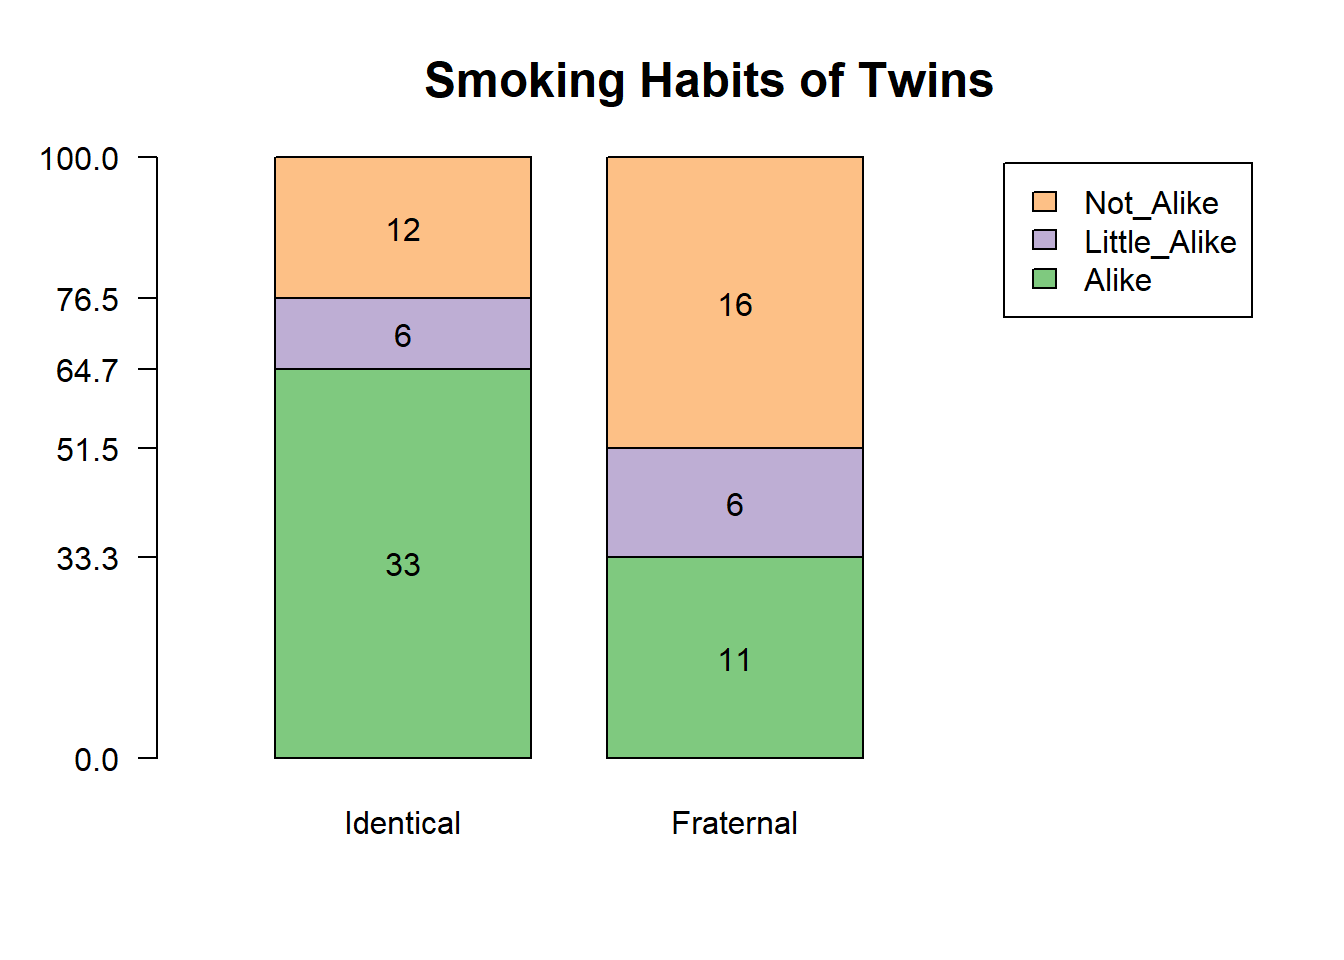
\includegraphics{Monty_Hall_ggplot_files/figure-latex/unnamed-chunk-5-1.pdf}

\begin{Shaded}
\begin{Highlighting}[]
\KeywordTok{monty_plot}\NormalTok{(}\DecValTok{30}\NormalTok{)}\OperatorTok{$}\NormalTok{p_wins}
\end{Highlighting}
\end{Shaded}

\begin{verbatim}
## [1] 0.7
\end{verbatim}

\hypertarget{repetitions}{%
\subsection{Repetitions}\label{repetitions}}

\begin{Shaded}
\begin{Highlighting}[]
\NormalTok{N2 <-}\StringTok{ }\DecValTok{10}
\NormalTok{m <-}\StringTok{ }\KeywordTok{list}\NormalTok{()}
\ControlFlowTok{for}\NormalTok{ (i }\ControlFlowTok{in} \DecValTok{1}\OperatorTok{:}\NormalTok{N2) \{}
\NormalTok{m[[i]] <-}\StringTok{ }\KeywordTok{monty_plot}\NormalTok{(}\DecValTok{30}\NormalTok{)}\OperatorTok{$}\NormalTok{monty}
\CommentTok{#> Title 에 몇 번째 시도인지 횟수 표시}
\NormalTok{m[[i]] <-}\StringTok{ }\NormalTok{m[[i]]}\OperatorTok{+}\StringTok{ }
\StringTok{  }\KeywordTok{ggtitle}\NormalTok{(}\KeywordTok{paste0}\NormalTok{(}\StringTok{"Replication No."}\NormalTok{, i))}
\CommentTok{# m[[i]]}
\CommentTok{#> 그림을 매번 출력하려면 print()를 반드시 실행시켜야 함.}
\KeywordTok{print}\NormalTok{(m[[i]])}
\NormalTok{\}}
\end{Highlighting}
\end{Shaded}

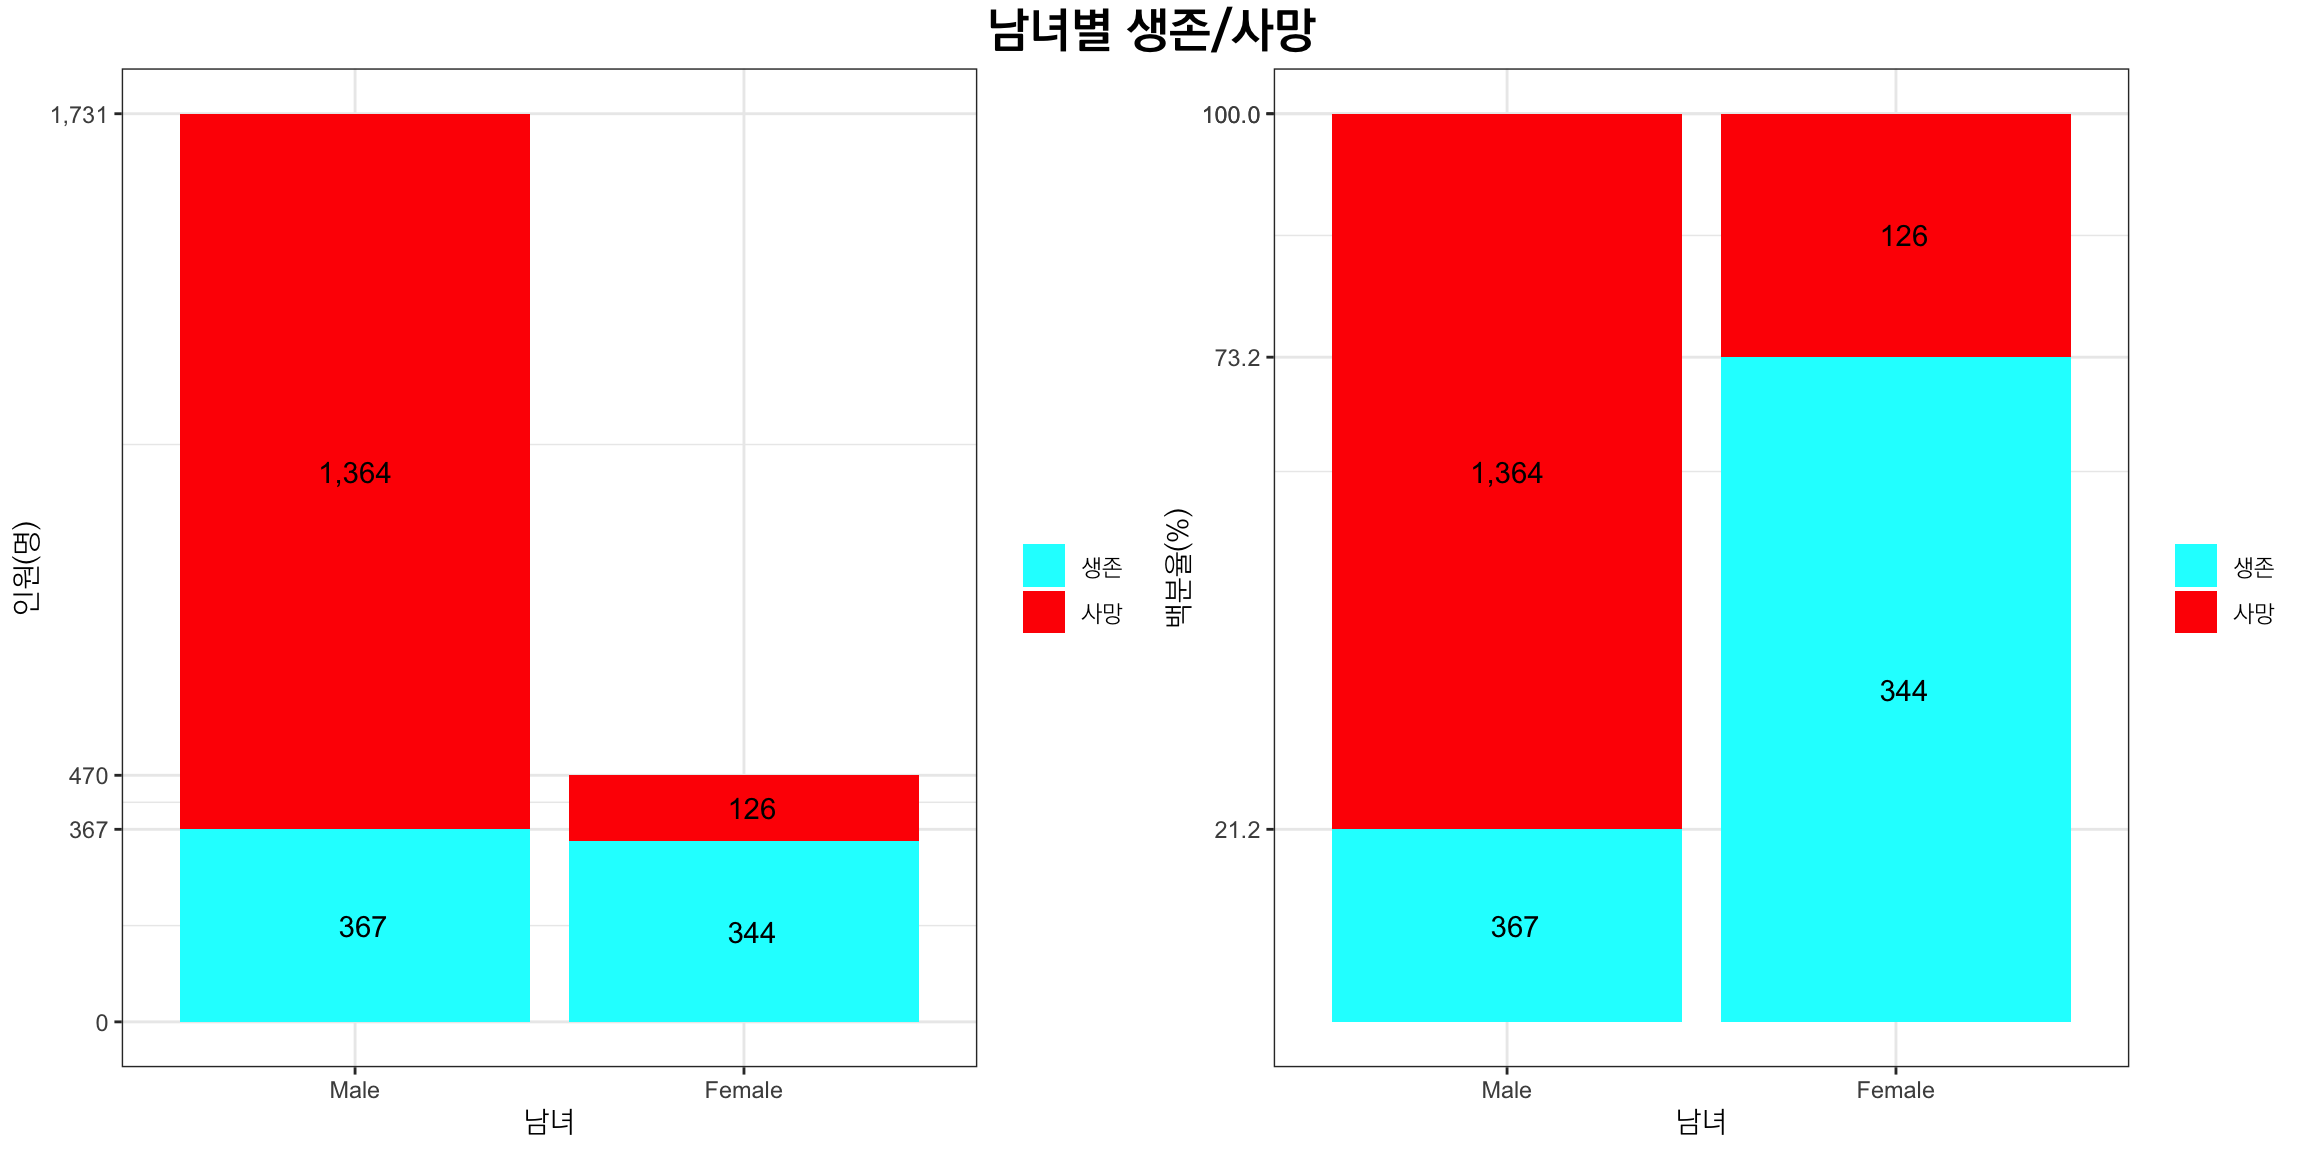
\includegraphics{Monty_Hall_ggplot_files/figure-latex/unnamed-chunk-6-1.pdf}
\includegraphics{Monty_Hall_ggplot_files/figure-latex/unnamed-chunk-6-2.pdf}
\includegraphics{Monty_Hall_ggplot_files/figure-latex/unnamed-chunk-6-3.pdf}
\includegraphics{Monty_Hall_ggplot_files/figure-latex/unnamed-chunk-6-4.pdf}
\includegraphics{Monty_Hall_ggplot_files/figure-latex/unnamed-chunk-6-5.pdf}
\includegraphics{Monty_Hall_ggplot_files/figure-latex/unnamed-chunk-6-6.pdf}
\includegraphics{Monty_Hall_ggplot_files/figure-latex/unnamed-chunk-6-7.pdf}
\includegraphics{Monty_Hall_ggplot_files/figure-latex/unnamed-chunk-6-8.pdf}
\includegraphics{Monty_Hall_ggplot_files/figure-latex/unnamed-chunk-6-9.pdf}
\includegraphics{Monty_Hall_ggplot_files/figure-latex/unnamed-chunk-6-10.pdf}

\begin{Shaded}
\begin{Highlighting}[]
\KeywordTok{print}\NormalTok{(m)}
\end{Highlighting}
\end{Shaded}

\begin{verbatim}
## [[1]]
\end{verbatim}

\includegraphics{Monty_Hall_ggplot_files/figure-latex/unnamed-chunk-6-11.pdf}

\begin{verbatim}
## 
## [[2]]
\end{verbatim}

\includegraphics{Monty_Hall_ggplot_files/figure-latex/unnamed-chunk-6-12.pdf}

\begin{verbatim}
## 
## [[3]]
\end{verbatim}

\includegraphics{Monty_Hall_ggplot_files/figure-latex/unnamed-chunk-6-13.pdf}

\begin{verbatim}
## 
## [[4]]
\end{verbatim}

\includegraphics{Monty_Hall_ggplot_files/figure-latex/unnamed-chunk-6-14.pdf}

\begin{verbatim}
## 
## [[5]]
\end{verbatim}

\includegraphics{Monty_Hall_ggplot_files/figure-latex/unnamed-chunk-6-15.pdf}

\begin{verbatim}
## 
## [[6]]
\end{verbatim}

\includegraphics{Monty_Hall_ggplot_files/figure-latex/unnamed-chunk-6-16.pdf}

\begin{verbatim}
## 
## [[7]]
\end{verbatim}

\includegraphics{Monty_Hall_ggplot_files/figure-latex/unnamed-chunk-6-17.pdf}

\begin{verbatim}
## 
## [[8]]
\end{verbatim}

\includegraphics{Monty_Hall_ggplot_files/figure-latex/unnamed-chunk-6-18.pdf}

\begin{verbatim}
## 
## [[9]]
\end{verbatim}

\includegraphics{Monty_Hall_ggplot_files/figure-latex/unnamed-chunk-6-19.pdf}

\begin{verbatim}
## 
## [[10]]
\end{verbatim}

\includegraphics{Monty_Hall_ggplot_files/figure-latex/unnamed-chunk-6-20.pdf}

\begin{Shaded}
\begin{Highlighting}[]
\NormalTok{Prop_Switching_wins_}\DecValTok{100}\NormalTok{ <-}\StringTok{ }\KeywordTok{replicate}\NormalTok{(}\DecValTok{100}\NormalTok{, }\KeywordTok{monty_plot}\NormalTok{(}\DecValTok{30}\NormalTok{)}\OperatorTok{$}\NormalTok{p_wins)}
\end{Highlighting}
\end{Shaded}

\hypertarget{stem-and-leaf}{%
\subsubsection{Stem and Leaf}\label{stem-and-leaf}}

\begin{Shaded}
\begin{Highlighting}[]
\KeywordTok{stem}\NormalTok{(Prop_Switching_wins_}\DecValTok{100}\NormalTok{)}
\end{Highlighting}
\end{Shaded}

\begin{verbatim}
## 
##   The decimal point is 1 digit(s) to the left of the |
## 
##   5 | 0003333
##   5 | 77777777
##   6 | 00000000000000000333333333333333333
##   6 | 777777777
##   7 | 0000000000000003333333333333
##   7 | 77777777
##   8 | 00003
\end{verbatim}

\end{document}
